\documentclass[final]{fhnwreport}       %[mode] = draft or final
                                        %{class} = fhnwreport, article, 
                                        %          report, book, beamer, standalone
%%---Main Packages-----------------------------------------------------------------------
\usepackage[english, ngerman]{babel}	%Mul­tilin­gual sup­port for LaTeX
\usepackage[T1]{fontenc}				%Stan­dard pack­age for se­lect­ing font en­cod­ings
\usepackage[utf8]{inputenc}				%Ac­cept dif­fer­ent in­put en­cod­ings
\usepackage{lmodern}                    %The newer Font-Set
\usepackage{textcomp}					%LaTeX sup­port for the Text Com­pan­ion fonts
\usepackage{caption}					%Customising captions in floating environments
\usepackage{graphicx} 					%En­hanced sup­port for graph­ics
\usepackage{float}						%Im­proved in­ter­face for float­ing ob­jects
\usepackage{ifdraft}                    %Let you check if the doc is in draft mode

%%---Useful Packages---------------------------------------------------------------------
\usepackage{color}						%Colour control for LaTeX documents
\usepackage[pdftex,dvipsnames]{xcolor}  %Driver-in­de­pen­dent color ex­ten­sions for LaTeX
\usepackage{csquotes}                   %Simpler quoting with \enquote{}
\usepackage{siunitx} 					%A com­pre­hen­sive (SI) units pack­age
\usepackage{listings}					%Type­set source code list­ings us­ing LaTeX
\usepackage[bottom]{footmisc}			%A range of foot­note op­tions
\usepackage{footnote}					%Im­prove on LaTeX's foot­note han­dling
\usepackage{verbatim}					%Reim­ple­men­ta­tion of and ex­ten­sions to LaTeX ver­ba­tim
\usepackage[textsize=footnotesize]{todonotes} %Mark­ing things to do in a LaTeX doc­u­ment
\usepackage{titling}					%Control over the typesetting of the \maketitle command

%%---Tikz Packages-----------------------------------------------------------------------
\usepackage{standalone}
\usepackage{tikz}
\usepackage{circuitikz}
\usetikzlibrary{arrows}
\usetikzlibrary{calc}
\usetikzlibrary{intersections}

%%---Math Packages-----------------------------------------------------------------------
\usepackage{amsmath}					%AMS math­e­mat­i­cal fa­cil­i­ties for LaTeX
\usepackage{amssymb}					%Type­set­ting symbols (AMS style)
%\usepackage{amstext}
%\usepackage{amsfonts}
%\usepackage{breqn}
\usepackage{array}						%Ex­tend­ing the ar­ray and tab­u­lar en­vi­ron­ments
\usepackage{amsthm}					%Type­set­ting the­o­rems (AMS style)

%%---Table Packages----------------------------------------------------------------------
\usepackage{tabularx}					%Tab­u­lars with ad­justable-width columns
%\usepackage{longtable}
\usepackage{multirow}					%Create tab­u­lar cells span­ning mul­ti­ple rows
\usepackage{multicol}					%In­ter­mix sin­gle and mul­ti­ple columns

%%---PDF / Figure Packages---------------------------------------------------------------
\usepackage{pdfpages}					%In­clude PDF doc­u­ments in LaTeX
\usepackage{pdflscape}					%Make land­scape pages dis­play as land­scape
\usepackage{subfig}					    %Fig­ures di­vided into sub­fig­ures

%%---Other Packages----------------------------------------------------------------------
%\usepackage{xargs}                     %De­fine com­mands with many op­tional ar­gu­ments


%%---Bibliography------------------------------------------------------------------------
\usepackage[style=ieee,urldate=comp,backend=biber,language=english]{biblatex}
\addbibresource{literature/Kryg_Artikel.bib}

\DefineBibliographyStrings{ngerman}{
	url         = [Online]\addspace Available: ,
	urlseen		= {Abrufdatum}
}

%%---Main Settings-----------------------------------------------------------------------
\graphicspath{{./graphics/}}			%Defines the graphicspath
\geometry{twoside=false}				    %twoside=false disables the "bookstyle"
\setlength{\marginparwidth}{2cm}
\overfullrule=5em						%Creates a black rule if text goes over the margins => debugging




%%---User Definitions--------------------------------------------------------------------
%%Tabel-Definitions: (requires \usepackage{tabularx})
\newcolumntype{L}[1]{>{\raggedright\arraybackslash}p{#1}}    %column-width and alignment
\newcolumntype{C}[1]{>{\centering\arraybackslash}p{#1}}
\newcolumntype{R}[1]{>{\raggedleft\arraybackslash}p{#1}}

%%---Optional Package Settings-----------------------------------------------------------
%Listings-Settings: (requires \usepackage{listings}) => Example with Matlab Code
%\lstset{language=Matlab,%
%    basicstyle=\footnotesize\ttfamily,
%    breaklines=false,%
%    morekeywords={switch, case, otherwise},
%    keywordstyle=\color{Blue},%
%    tabsize=2,
%    %morekeywords=[2]{1}, keywordstyle=[2]{\color{black}},
%    identifierstyle=\color{Black},%
%    stringstyle=\color{Purple},
%    commentstyle=\color{Green},%
%    showstringspaces=false,%without this there will be a symbol in the places where there is a space
%    numbers=left,%
%    numberstyle={\tiny \color{black}},% size of the numbers
%    numbersep=9pt, % this defines how far the numbers are from the text
%    %emph=[1]{word1, word2,...},emphstyle=[1]\color{red}
%}							

% Eingefügt für C-Code Style
\renewcommand\lstlistingname{Codeausschnitt}
\lstset{language=C,
	basicstyle=\ttfamily,
	keywordstyle=\color{blue}\ttfamily,
	stringstyle=\color{red}\ttfamily,
	commentstyle=\color{green!70}\ttfamily,
	morecomment=[l][\color{magenta}]{\#}
}

%Hurenkinder und Schusterjungen verhindern (kein Scherz, Google es)
\clubpenalty10000
\widowpenalty10000
\displaywidowpenalty=10000	



%Titel mit Mathematik immer fett drucken
\usepackage{sectsty}
\allsectionsfont{\boldmath}




			                %loads all packages, definitions and settings											
\title{Differentielle Kryptoanalyse}  		        %Project Title
%\author{Team 1}      				    %Document Type => Technical Report, ...
%\date{\today}          				%Place and Date

\begin{document}

%%---TITLEPAGE---------------------------------------------------------------------------------
\thispagestyle{empty}
%	\ohead{\includegraphics[scale=0.5]{Bilder/Logo_FHNW.jpg}}
	\begin{figure}
		 \vspace*{-\topskip}\vspace*{-\headsep}
		
\includegraphics[scale=1]{graphics/fhnw_ht_logo_de.pdf}
	\end{figure}

	
	\begin{center}
		\vspace*{2cm}
		{\huge{\textbf{\thetitle}}}\\
		\vspace*{0.5cm}
		
		{\scshape\Large Artikel Kryptographie \\} 
		\Large{Windisch, \today}
		
		\vspace*{-1cm}						    %compensates the space after the date line.
		\vfill
		\begin{figure}[H]
		\centering
		
\includegraphics[width=0.5\textwidth]{Titelbild.png}
		\cite{thirah_vorhangeschloss-schlussel-computer-icons_nodate}
		%\raggedleft
		\end{figure}
		
	
		\vfill
		
		\begin{normalsize}
			{
			\renewcommand\arraystretch{2}
			\begin{tabular}{>{\bf}p{4cm} l}
			Autoren   		           & 	Gabriel Nussbaumer und Fabian von Büren\\
			Dozent                 &    Dr. M. Hufschmid\\
			Modul		               &    Kryptographie (kryg)\\
			Hochschule                 &    Hochschule für Technik - FHNW\\
			Studiengang                &    Elektro- und Informationstechnik\\
%			Version                    &    1.0 %Normally not used!
			\end{tabular}
			}
		\end{normalsize}
	\end{center}
\clearpage
			
%%---ABSTRACT----------------------------------------------------------------------------
%\selectlanguage{english}				%ngerman or english
%\thispagestyle{empty}
%\begin{abstract}

Smart Home is the automation, and data-based control of electronic devices and light energy systems in your own home. This report is about a smart home system solution with MQTT communication. The development of an actor board with different switching possibilities, where electronic devices are connected, as well as the development of a touch sensor board with temperature measurement are described. A closed system with its own MQTT-broker is completed with the server software.The server software enables a perfect interaction between the components and the integration of a language assistant. The whole system can be integrated with existing Smart Home and offers cross-platform compatibility with other solutions.


%Der Softwareteil befasst sich mit verschiedenen Komponenten, so wird ein Framework für den Sensor/Aktorbaustein wie auch das Framework für den Inhouse Server und das MQTT Konzept beschrieben. Das Hardwarekonzept des Sensorbausteins besteht im wesentlichen aus einem WiFi fähigen Mikrocontroller, einem Temperatursensor, Buttons und LEDs. Dabei besteht der Sensorbaustein aus drei physisch getrennten Teilen: der Spannungsversorgung, dem Hauptprint und der Frontprint. Der Frontprint beinhaltet Touchsensoren und LEDs, welche einen individualisierten Einschaltzustand, z.B Lüftung ist an, signalisieren. Das wichtigste im Aktorbaustein ist ebenso ein Mikrocontroller mit WiFi, dazu kommen noch Relais, $10\;V$ Ein-/Ausgänge und LEDs, um den Schaltzustand der Relais zu signalisieren.

%Das Abstract ist eine Art Zusammenfassung des ganzen Dokuments. Es gibt einen Einblick in die Aufgabenstellung, wie diese umgesetzt wurde und welches Ergebnis erreicht wurde. Aus diesem Grund wird das Abstract immer ganz am Schluss der Arbeit verfasst. Es besteht aus einem zusammengehörenden Absatz und umfasst ungefähr 10 bis 20 Zeilen.Formeln, Referenzen oder andere Unterbrechungen haben im Text nichts zu suchen.Direkt unter dem Abstract folgt eine Liste von drei bis vier Stichworten/Keywords. Diese werden in alphabetischer Reihenfolge aufgelistet und beschreiben das Themengebiet der Arbeit.

%\vspace{2ex}
%\textbf{Keywords: Anleitung, LaTeX, Thesis, Vorlage}
\end{abstract}	


%%---TABLE OF CONTENTS-------------------------------------------------------------------
\pagenumbering{Roman}		
\selectlanguage{ngerman}				%ngerman or english
\tableofcontents
\clearpage

%%---TEXT--------------------------------------------------------------------------------
\pagenumbering{arabic}

\section{Einleitung} 
Für eine integrale Raumautomation müssen alle beteiligten Gewerke geregelt werden, dazu gehören: Beschattung, Licht, Heizung, Lüftung und Klima.
Der Auftraggeber möchte eine möglichst preisgünstige Sensor/Aktor-Plattform um jene integrale Raumautomation zu ermöglichen. Bisher wurde die Idee, verschiedene Sensoren und Aktoren über IOT miteinander auszulesen bzw. zu steuern, in der Raumautomations-Branche verwirklicht, jedoch hat es sich als schwierig erwiesen solch eine anwendungsfreundliche Plattform, wie sich der Auftraggeber gewünscht hat, käuflich zu erwerben. Um die Situation zu verbessern soll eine Plattform auf Basis eines Single-Chip-uC, welcher Ein- und Ausgänge sowie ein Sensor-Baustein beinhalten realisiert werden. Zusätzlich möchte man mithilfe eines MQTT-Brokers die IOT-Geräte verbinden. Die Erstinbetriebnahme der Plattform soll mit Hilfe eines Web-Interface ablaufen, wofür das Gerät erstmal als WiFi Access-Point auf startet. 
Die folgende Tabelle \ref{tab: Ausgangslage} fasst die Anforderungen an das System zusammen.
\begin{table}[h!]
	\centering
	\begin{tabular}{|c|l|}
		\hline
		\textbf{\begin{tabular}[c]{@{}c@{}}Aktor\\   Baustein\end{tabular}} & \begin{tabular}[c]{@{}l@{}}\textbullet 4 Relais Schaltspannung 230 V\\ \textbullet 2 Ausgänge 0-10 V\\ \textbullet 2 Eingänge 0-10 V\\ \textbullet Netzwerkschnittstelle\\ \textbullet 24 VDC Versorgungsspannung\end{tabular} \\ \hline
		\textbf{Sensor Baustein}                                            & \begin{tabular}[c]{@{}l@{}}\textbullet 4 Taster\\ \textbullet Netzwerkschnittstelle\\ \textbullet Geometrie: Standard Lichtschalter\\ \textbullet 5 VDC Versorgungsspannung\end{tabular}                                       \\ \hline
		\multicolumn{1}{|l|}{\textbf{Kommunikation}}                        & \begin{tabular}[c]{@{}l@{}}\textbullet MQTT Broker\\ \textbullet WEB Interface\\
		\textbullet Sprach Assistent\end{tabular}                                                                                                                                   \\ \hline
	\end{tabular}
	\caption{Ausgangslage}
	\label{tab: Ausgangslage}
\end{table}
%\clearpage
\section{Historisches}\label{sec:Historisches}








%\clearpage
\section{Funktionsweise}\label{sec:Funktionsweise}










%\clearpage
\section{Sicherheit}\label{sec:Sicherheit}










\section{Schluss}

\subsection{Reflektion}

In diesem Kapitel werden die Projekt Ziele Reflektiert. In der untenstehenden Tabelle \ref{tab: Teilziele} sind die zu beginn des Projekts Definierten Teilziele so wie der Status, in welchem der Fachbericht am ende verfasst wurde.
\begin{table}[h!]
	\small
	\begin{tabular}{|c|l|c|}
		\hline 
		Definition & Status \\ 
		\hline 
		Sensor- und Aktorbaustein sind als Prototypen hergestellt& Erfüllt \\ 
		\hline 
		Analyse und Evaluation Mikrocontroller & Erfüllt \\ 
		\hline 
		Frameware ist kompilierbar und erlaubt eine Inbetriebnahme der Prototypen & Erfüllt \\ 
		\hline 
		Signalverknüpfungen sind mit OpenHab realisierbar & Erfüllt \\ 
		\hline 
		Sensor- und Aktorbaustein sind optimiert (Redesign), Mechanisches Gehäuse ist erstellt  & Erfüllt \\ 
		\hline 
		Systemeinrichtung gestaltet sich Benutzerfreundlich & Erfüllt \\ 
		\hline 
		Validierung des gesamten Systems, Testergebnisse sind Dokumentiert n & Erfüllt \\ 
		\hline 
		Befehle können mit Sprachsteuerung ausgeführt werden & Erfüllt \\ 
		\hline 
		Dokumentation abgeschlossen & Erfüllt \\ 
		\hline 
		\end{tabular}
	\caption{Teilziele}
	\label{tab: Teilziele}	 
\end{table}



\subsubsection{Fazit}
 In diesem Projekt wurden Erfahrungen gewonnen, wie eine Hardware Lösung für eine IOT-Anwendung aussehen kann. Es gab einige Probleme wegen des verwendeten Mikrocontrollers, insbesondere des ADCs. Es wurde darauf verzichtet einen externen ADC zu verwenden und andere Lösungen gesucht, sowie die möglichen Verbesserungen der momentanen Lösung erarbeitet. Es hat sich darüber als schwierig herausgestellt, die Temperatur exakt zu messen, da die Umgebungsbedingungen anders sein können, wie stehende Luft und erwärmende Frontplatte. Weitere Erkenntnisse wurden ebenfalls im Bereich des Google Assistent gewonnen, durch die dynamische DNS Adresse  und SSL-Zertifikate gestaltete sich die Integration nicht mit einer direkten Verbindung, siehe Kapitel Sprachassistent.


\pagebreak


%\clearpage
%%---BIBLIOGRAPHY------------------------------------------------------------------------


{\sloppypar
%\printbibliography[heading=bibnumbered ]
\label{sec:lit}
\selectlanguage{ngerman}				%ngerman or english
\printbibliography
}

%\pagebreak

%\input{sections/8_0_Ehrlichkeitserklaerung}
%\pagebreak
%%---APPENDIX----------------------------------------------------------------------------
%\appendix
%\begin{appendix} %Anhang
	\section{Anhang Benutzerhandbuch}

%\includepdf[pages={1-2},nup=1x2,landscape=true,scale=0.85,offset=10 -40,pagecommand={\section{Eingefügtes Dokument; zwei Seiten auf einer}\label{app:Aufgabenstellung}\thispagestyle{myheadings}}]{appendix/aufgabenstellung.pdf} \newpage

%%Bei mehrseitigen Dokumenten die folgenden Seiten ohne Überschrift:
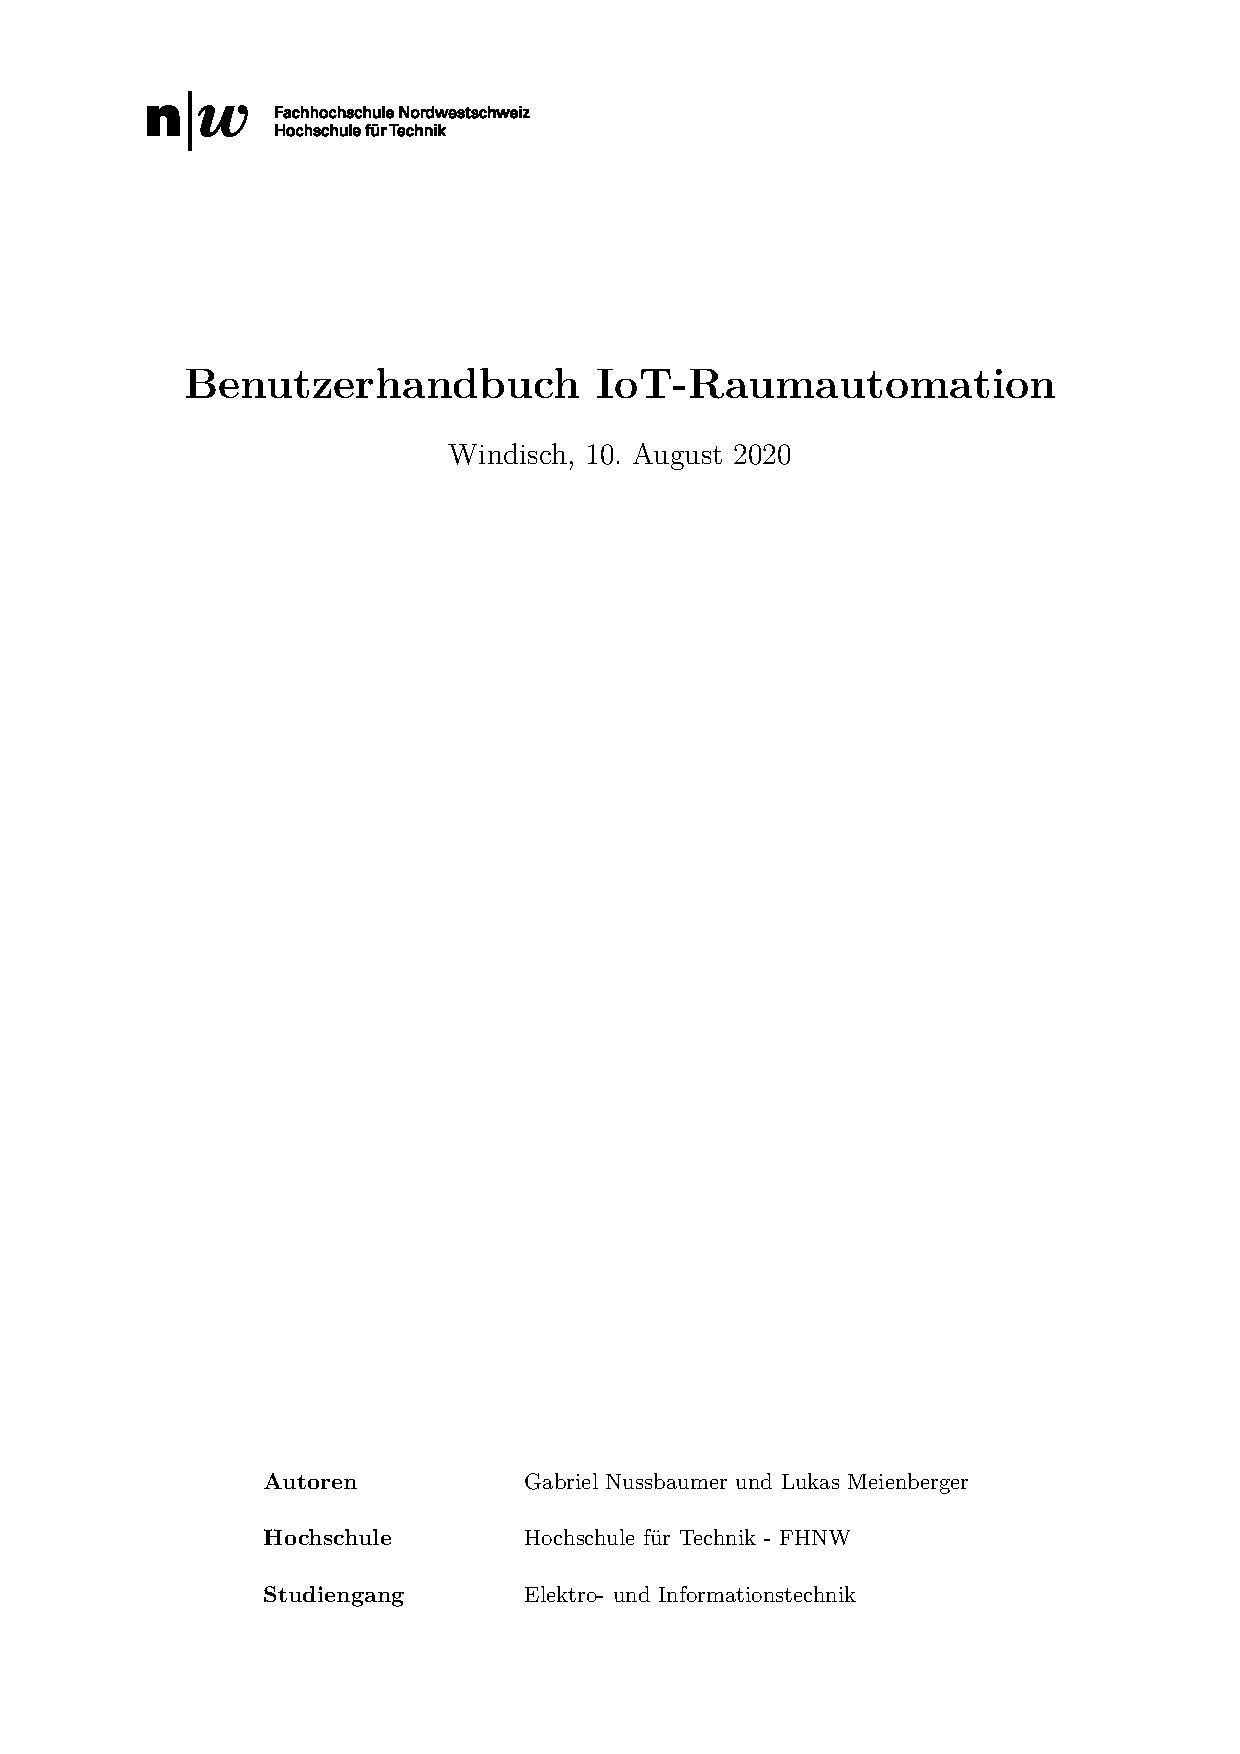
\includepdf[pages=-]{Benutzerhanndbuch.pdf} \newpage

%\includepdf[pages={1},nup=1x1,landscape=true,scale=0.85,offset=10 -40,pagecommand={\section{Eingefügte PDF-Tabelle}\label{app:Timetable}\thispagestyle{myheadings}}]{appendix/timeline_example.pdf} \newpage

%%Bei mehrseitigen Dokumenten die folgenden Seiten ohne Überschrift:
%\includepdf[pages={2-5},nup=1x1,landscape=true,scale=0.85,offset=0 -20,pagecommand={\thispagestyle{myheadings}}]{appendix/timeline_example.pdf} \newpage

\end{appendix}


%%---NOTES for DEBUG---------------------------------------------------------------------
%\ifdraft{%Do this only if mode=draft
%\usepackage{todonotes})
%\newpage
%\listoftodos[\section{Todo-Notes}]
%\clearpage
%}
%

\end{document}
